\documentclass{article}\usepackage[]{graphicx}\usepackage[]{color}
%% maxwidth is the original width if it is less than linewidth
%% otherwise use linewidth (to make sure the graphics do not exceed the margin)
\makeatletter
\def\maxwidth{ %
  \ifdim\Gin@nat@width>\linewidth
    \linewidth
  \else
    \Gin@nat@width
  \fi
}
\makeatother

\definecolor{fgcolor}{rgb}{0.345, 0.345, 0.345}
\newcommand{\hlnum}[1]{\textcolor[rgb]{0.686,0.059,0.569}{#1}}%
\newcommand{\hlstr}[1]{\textcolor[rgb]{0.192,0.494,0.8}{#1}}%
\newcommand{\hlcom}[1]{\textcolor[rgb]{0.678,0.584,0.686}{\textit{#1}}}%
\newcommand{\hlopt}[1]{\textcolor[rgb]{0,0,0}{#1}}%
\newcommand{\hlstd}[1]{\textcolor[rgb]{0.345,0.345,0.345}{#1}}%
\newcommand{\hlkwa}[1]{\textcolor[rgb]{0.161,0.373,0.58}{\textbf{#1}}}%
\newcommand{\hlkwb}[1]{\textcolor[rgb]{0.69,0.353,0.396}{#1}}%
\newcommand{\hlkwc}[1]{\textcolor[rgb]{0.333,0.667,0.333}{#1}}%
\newcommand{\hlkwd}[1]{\textcolor[rgb]{0.737,0.353,0.396}{\textbf{#1}}}%

\usepackage{framed}
\makeatletter
\newenvironment{kframe}{%
 \def\at@end@of@kframe{}%
 \ifinner\ifhmode%
  \def\at@end@of@kframe{\end{minipage}}%
  \begin{minipage}{\columnwidth}%
 \fi\fi%
 \def\FrameCommand##1{\hskip\@totalleftmargin \hskip-\fboxsep
 \colorbox{shadecolor}{##1}\hskip-\fboxsep
     % There is no \\@totalrightmargin, so:
     \hskip-\linewidth \hskip-\@totalleftmargin \hskip\columnwidth}%
 \MakeFramed {\advance\hsize-\width
   \@totalleftmargin\z@ \linewidth\hsize
   \@setminipage}}%
 {\par\unskip\endMakeFramed%
 \at@end@of@kframe}
\makeatother

\definecolor{shadecolor}{rgb}{.97, .97, .97}
\definecolor{messagecolor}{rgb}{0, 0, 0}
\definecolor{warningcolor}{rgb}{1, 0, 1}
\definecolor{errorcolor}{rgb}{1, 0, 0}
\newenvironment{knitrout}{}{} % an empty environment to be redefined in TeX

\usepackage{alltt}

\title{Temperature and the Santa Ana Sucker}
\author{Sophie Janssen and Nicole Larson}
\IfFileExists{upquote.sty}{\usepackage{upquote}}{}
\begin{document}


\maketitle

\newpage
\tableofcontents
\newpage

\section{Introduction}

\subsection{Problem Statement}

This experiment aims to see the true impact of fluctuating water temperature Santa Ana sucker (C. santaanae) population in the Rialto portion of the Santa Ana river in Southern California. Populations of the Santa Ana sucker have been declining and in peril since the mid-1950s, however the lack of attention and careful actions have lead to its continued demise. The experiment has gathered water temperature data in four portions of the Santa Ana river, extending less than a mile along the river. Our original research question was how does temperature affect the Santa Ana Sucker? Our null hypothesis was that the Santa Ana Suckers will be spread randomly through the river, without regard to possible temperature differences. There will also be no noticeable temperature abnormalities in the river. After collecting data and recognizing noticeable daily spikes in temperature, we expanded on our question to include several more driving questions regarding the relationship between water temperature and the Santa Ana sucker: does the frequency of temperature drops and spikes affect the sucker population and if so, in what way? Which portions of the river contain the most Santa Ana suckers and how much is this a result of the fluctuating temperatures? Is the Rialto plant contributing to the temperature spikes or can these fluctuations be written off as typical of the weather during these weeks? We expect the fish to stick to water that is at their optimum temperature, which is under 22 degrees Celsius, or to temperatures reasonably close to that. 

\subsection{Background}

From our background research, we found that many species of fish are affected by the temperature in their habitats. Higher water temperatures can cause nondirectional sex reversal, the release of chemical factors in the water, disruption of the endocrine system of the fish, death of critical microbes due to algal blooms, depleted oxygen levels, and even high rates of mortality (Coulter, et. al, 2015). For the Chinook salmon in the Mercer river, restoration efforts have been thwarted by higher temperatures and minimal riparian cover, despite gains in water quality, flow, and reintroduction of the species (Albertson, et. al, 2012). Fish in the Trent river experienced higher water temperatures and migrated away from their preferred spawning and developing grounds, leading to further drops in population and the expansion of a dead zone (Sadler, 1980). These studies allowed us to see that the Santa Ana river is undergoing changing conditions very similar to many other rivers, and that the junction of the treated water and river bed should be investigated more closely. The Santa Ana River has been reduced to a small stream at our sites and thus, large influxes of treated wastewater from the Rialto Channel and the Rix Influx have a significant impact on the health of the ecosystem being the primary source of water. Daily temperature fluctuations could have an impact on the Santa Ana Suckers as well, as the water could range in temperature so much as to completely destroy the life cycle of the sucker. According to research done by the US Fish and Wildlife Service (2012), mortality rates rise significantly when water temperatures exceed 32.8 degrees Celsius, which would put this already depleted population in further jeopardy. The fish stick to water that is at their optimum temperature, which is under 22 degrees Celsius, or migrate to locations that have temperatures close to that. Sucker migration which could affect other aspects of the ecosystem and create dead zones as well as overpopulated regions which may compete with each other for limited resources, further stressing out the surviving endangered specimens. 
 
\subsection{Background Research w/Citations} 

Albertson, L.K., Koenig, L.E., Lewis, B.L., Zeug, S.C., Harrison, L.R., \& Cardinale, B.J. (2012). How Does Restored Habitat for Chinook Salmon (Oncorhynchus Tshawytscha) in the Merced River in California Compare with other Chinook Streams? River Research and Applications, 29(4), 469-482). doi: 10.1002/rra.1604

By looking at Chinook salmon in the Merced river, restoration projects seemed to be failing to prevent the Chinook population from falling. The installation of gravel augmentation in a reconfigured channel seemed to have little impact on the salmon, suggesting that other factors were catalyzing the fall of the species. By comparing the restored portion with other portions of the Merced river, food web characteristics and flow discharge seemed to produce the same results on the various life stages of the salmon. However, higher temperatures, less woody debris, and minimal riparian cover seemed to limit populations in the restored portions. Restoration efforts are then presented with an added challenge of ensuring that every aspect of the ecosystem is beneficial to the species, which demands more work toward temperature regulation and attempts to restore the river bank. To see how the Santa Ana sucker would react to similar conservation efforts would be interesting in discussions in attempting to determine solutions. 

Coulter, D. P., Höök, T. O., Mahapatra, C. T., Guffey, S. C., \& Sepúlveda, M. S. (2015). Fluctuating Water Temperatures Affect Development, Physiological Responses and Cause Sex Reversal in Fathead Minnows. Environmental Science \& Technology, 49(3), 1921-1928. doi:10.1021/es5057159

Human activities can increase water temperature. Water-based organisms are sensitive to temperature change, especially young fish due to limited mobility. This paper explained how young Flathead Minnows exposed to warmer temperatures underwent a nondirectional sex reversal. This paper shows us how temperature can greatly affect fish and stress them out. Clearly, water temperature drastically affects fish, not necessarily in a positive way, and therefore, we should see if there is a correlation between stream temperature and where the Santa Ana Sucker chooses to live.

Los Huertos, Marc. (2016). Thermal Properties of Water. Environmental Science of Aquatic Systems. 297-308.

Temperature varies greatly in its impact on fish depending upon the conditions affecting the lake or river. Heat, temperature, thermal energy, and heat capacity all slightly change how heat is measured in an ecosystem. Water in general has a high heat capacity, which indicates its high specific heat. These aquatic systems therefore often retain their heat and are less susceptible to increase/decrease in temperature. Inflows/mixing can have an effect on water temperature but it is often hard to detect due to thermal stratification mixing, seasonal change in temperature profile depth, and small volume inflow in terms of fraction of the lake volume. This chapter sheds light that variations in temperature trigger chemicals dissolving/remaining, tend to raise/lower a fish’s body temperature to the same degree, etc. Temperature impacts many other features of water quality, which will be important to keep in mind going forward with the project.

Sadler, K. (1980). Effect of the warm water discharge from a power station on fish populations in the river Trent. Journal Of Applied Ecology, 17(2):349-357.

A power station discharged water that was on average 7 degrees Celsius above normal in the River Trent. This meant that in affected areas, the winter migration was delayed from Sep/Oct to Dec/Jan, while in unaffected areas, migration continued at normal times. Also, below the power station, fish preferred to live further downstream, in terms of diversity and population density. This tells us that fish are able to change their living patterns based on water temperature, and shows that fish were noticeably affected by the temperature change. 

U.S. Fish \& Wildlife Service. 2012. Recovery Outline for Santa Ana sucker. Sacramento, California. 38 pp.

This report discusses Santa Ana Suckers and possible recovery plans. In order to do so, it clearly outlines Sucker habitat preferences, behavior, and threats. We used this source to determine preferred temperature for the Santa Ana Sucker and in general to inform ourselves more about the fish. Little research has been done on specific threats to the Santa Ana Sucker, but the document did point out possible threats arising from hydrological modification and urban development in general. Sophie and I thought that potentially water coming out of a treatment plant could be a threat under hydrological modification or urban development, so that will be what our research focuses on.

\subsection{Objectives}

Our goal was to find out whether or not temperature was affecting the population and/or livelihood of the Santa Ana Sucker in the Santa Ana River. Our null hypothesis was trifold:


  1. The Santa Ana Suckers will be spread randomly through the river, without regard to possible differences in temperature. 
  2. There will also be no noticeable temperature abnormalities in the river. In other words, the Veolia water treatment plant at Rialto does not significantly contribute to water temperature fluctuations/overall average temperature. 


If this null hypothesis is found untrue, due to a correlation between temperature and fish populations, as well as measurable temperature change caused by the treatment plant, the U.S. Fish and Wildlife Service should follow up with the Rialto water facility to better regulate temperature and depth of the river. Also, conservation efforts should extend beyond pollution control and habitat protection to include temperature regulation to ensure that the habitat that is being protected is totally habitable.

\section{Methods}

\subsection{Site Description}

This data was collected in the Rialto portion of the Santa Ana river over a period of eleven nights for locations 1, 3, and 4, and seven nights for location 2. Location 4 was the plunge pool, located the furthest downstream. Location 3 was where the Rix influx was. Location 2 was upstream below the concrete channel and Location 1 was in the concrete Rialto channel. The pendant data logger collected data in degrees Celsius every fifteen minutes from 9/24/16 through 10/05/16, or until 10/1/16 for Location 2. 

\begin{figure}
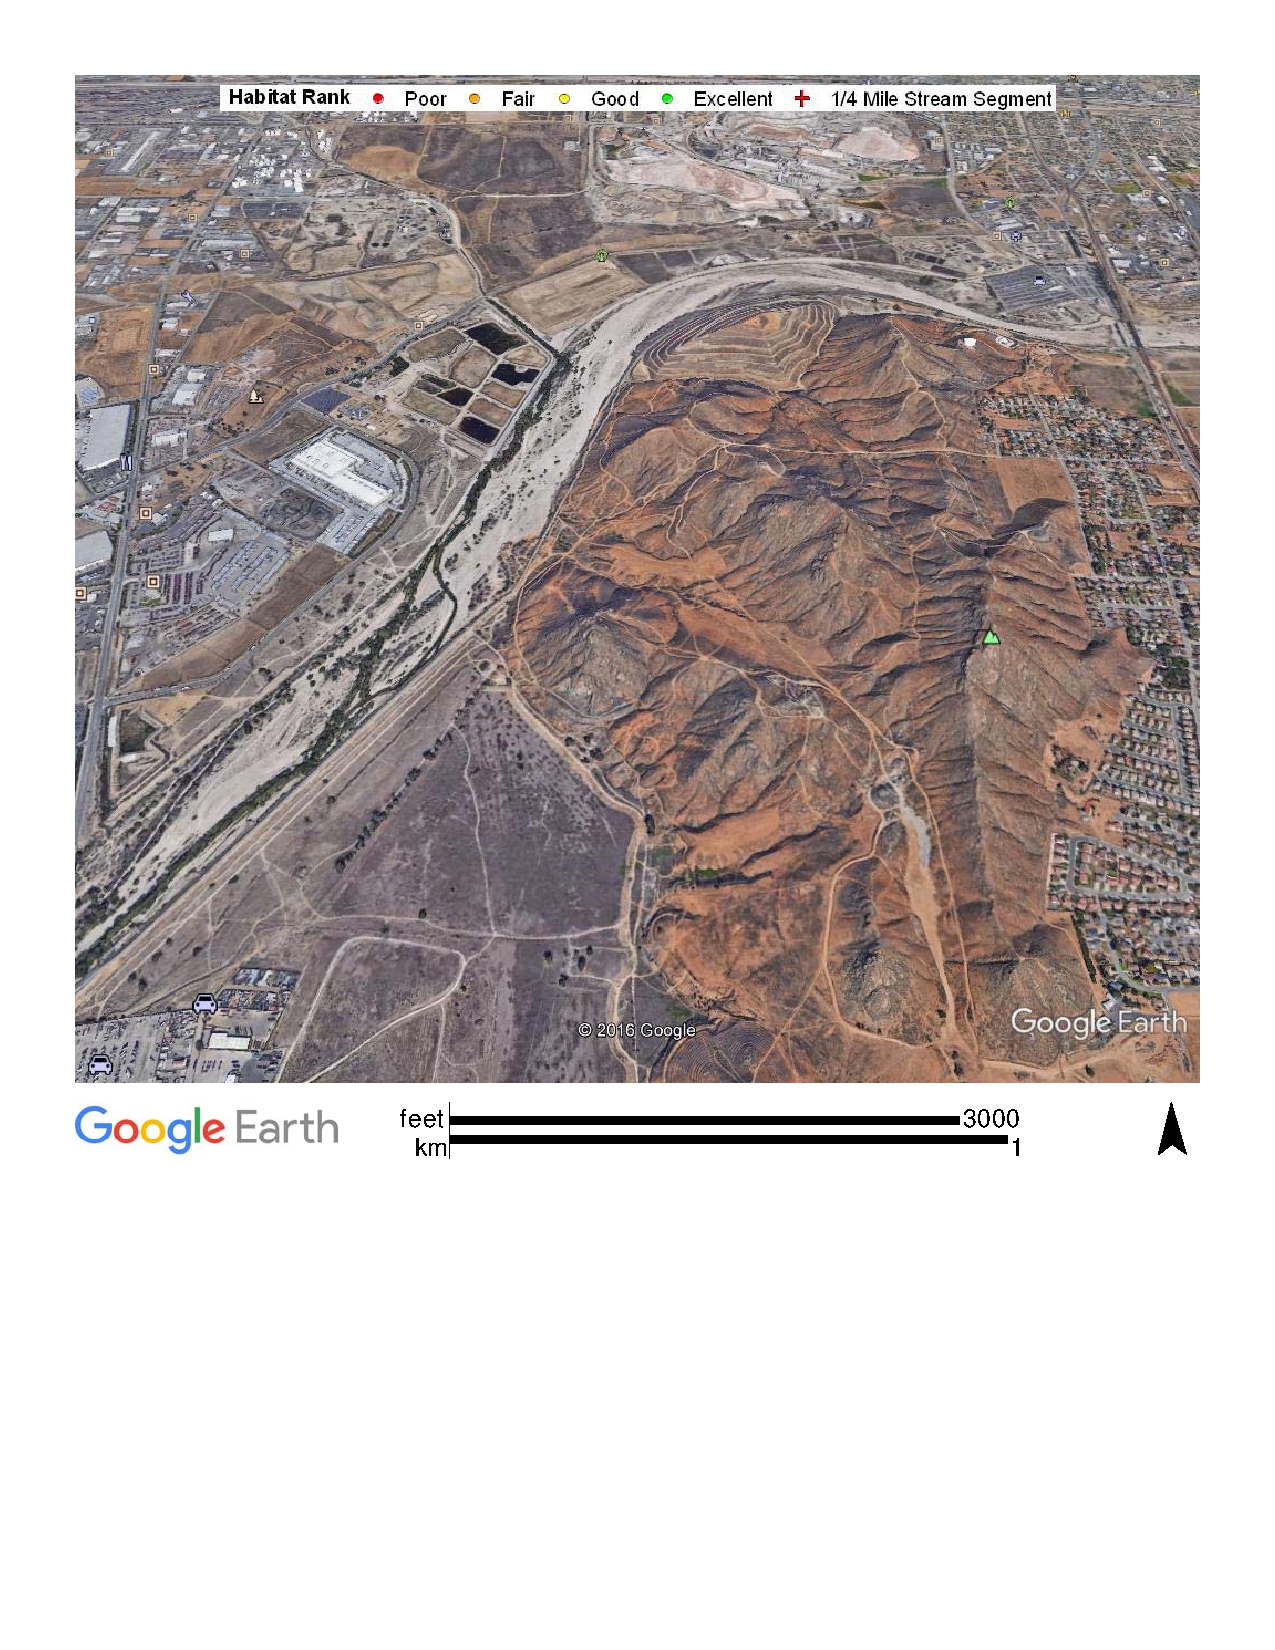
\includegraphics[width=1.00\textwidth]{Figures/SantaAna_SatelliteImage}
\caption{Google Earth --Example of a map. What's wrong with this image?}
\label{SAR_Image}
\end{figure}

\subsection{Materials and Equipment}

4 HOBO Tidbit Water Temperature Data Logger,
1 Optic USB U-4 Base Station,
1 Coupler,
4 Green Garden stakes,
Red flags,
Yellow marking tape,
Free HOBOware software,
Transportation to and from the river,
Ice Bath

\subsection{Procedure}

We obtained four HOBO Tidbit water temperature Data Loggers to set up at the Rialto Channel at Agua Mansa (site 1), another at the point where the Rix Influx meets the river (site 3), another just above that site (site 2), and a fourth in the pool where Suckers have previously been observed (site 4). Before going to the river, we programmed the loggers via our base station and the HOBOware software to collect water temperature data every 15 minutes. In order to start the data process, we put each logger into the coupler and pushed the level til the light was flashing. We then put them in the river by looping a garden stake through one, sticking it into the substrate, and securing it with rocks. We then put yellow marking tape on plants nearby and red flags along the bank to show where we left the main path. We repeated this for each site, making sure the loggers were secure and fairly hidden. After seven nights (for site 2) and eleven nights (for the other sites), we returned to the river and collected the loggers. In the lab, using the software, we loaded our data and transferred it to RStudio. Later, to calibrate the loggers, we put them in an ice bath for 6 minutes to ensure that the temperature settled around zero and each logger was measuring to the same temperature with the same accuracy.

\subsection{Field Methods} 

At each location, we used a garden stake to secure a logger in the river. We then marked the location using yellow marking tape and used red flag stakes in order to remember where in the river we left the loggers. We also secured the loggers using rocks to ensure they were less visible and would remain in place for a week. Later, we collected them and removed our flags and marking tape. 

\subsection{Laboratory Methods}

In the lab, we used an ice bath to calibrate the loggers. To do this, we put the loggers in an ice bath and left them there for an hour. We then checked to see what data they were reading. Ideally, if calibrated correctly, it would have been 0 degrees Celsius. All the loggers were calibrated within .2 degrees.

\subsection{Statistical Methods}

We used HoboWare to collect the data off the loggers, then moved it to Excel, clipped it appropriately, and made a graph and charts using r studio. 

\section{Results}

  We found that temperature fluctuated between a minimum of 25.12 degrees Celsius and a maximum of 31.37 degrees Celsius, which are all well above the 22 degrees that many studies found is the optimal temperature for the fish. The plunge pool, site 4, contained the most data points around 27.5 degrees, which proved true for each locations, having the most repetitive temperature between 27 and 28 degrees. Site 4, however, had the least temperature range, only varying between 27 and 28.5 degrees, while other sites tended to have a bigger variation of almost 6 degrees. 
  
(Figure \ref{Temp}).

\begin{figure}
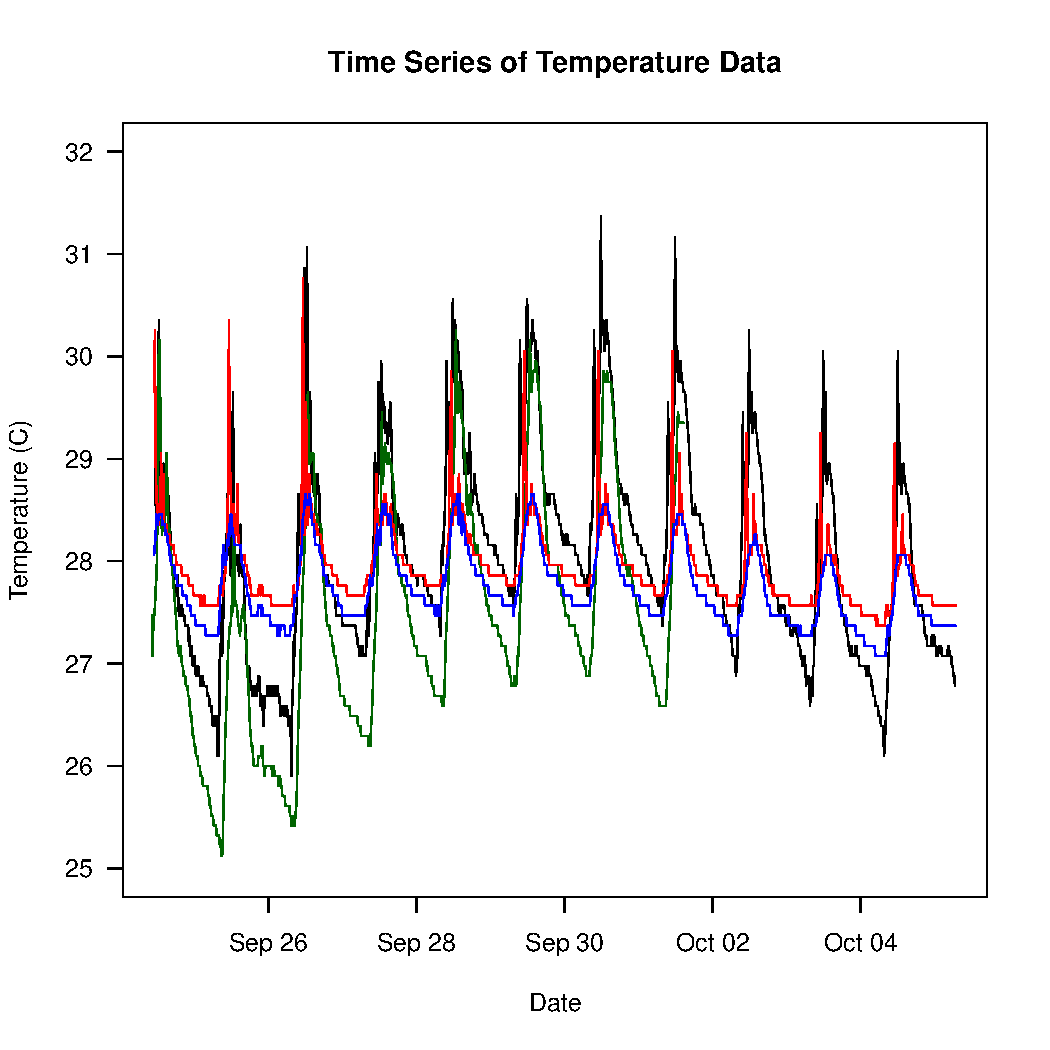
\includegraphics{Figures/Temp}
\caption{Temperature time...}
\label{Temp}
\end{figure}

\section{Discussion}

The temperature data suggests that there is something abnormal happening in the river. There were pretty extreme spikes, especially at sites 1 and 2. Our original hypothesis when we saw this was to assume water spikes were occurring from the Rialto Channel and as they travelled down river, becoming less extreme. However, when we looked at the timing of these spikes, they did not correlate with each other, and the spikes further downstream were actually occurring before the spikes upstream. We found that there were indeed daily spikes and lows in temperature. Site 1 and Site 2 had especially dramatic spikes, with Site 1 fluctuating up to 5.41 degrees a day. We are unsure why this happened for the Santa Ana river where the farthest location from the Rialto channel contained the most fluctuations. In terms of fish population, using the data from the Fish and Wildlife Service, as well as the data from Clare and Wendy's group, we realized that there were no fish counted at site 1, only one fish counted in the afternoon at site 2 at various points, no fish were found by the FWS at site 3, but many fish were observed by Clare and Wendy in the plunge pool at site 4. The data collected by Clare and Wendy’s group may not have been a very good indicator of population because the fish were constantly swimming around and only the fish in the foreground during the hours of videoing were counted. However, this does tell us that in general the fish were more abundant downstream, where the least extreme temperature spikes were occurring. From what we observed, the extreme temperature spikes at sites 1 and 2, and the medium spike at site 3, could have caused the fish to prefer to stay at site 4, where they are most abundant. This disproves our null hypothesis that the fish would be randomly spread throughout the channel and that temperature would remain fairly constant throughout the river, which suggests there could be a correlation between what is happening temperature wise and with the location of the suckers.

\section{Conclusion and Recommendations}

We collected our data in a simple yet straightforward manner to ensure its comprehensibility and communicability. Not only does our data span over a week, 24 hours a day, but we collected at four different sites every 15 minutes, giving us a significant spread of data to work with. To garner the most accurate results, we would have preferred to take measurements annually and compared them, in order to determine the causation of the oscillating fish populations more directly.  Given the limited timeline of the experiment, our data can be said to have captured a glimpse into an average week for this portion of the river, and can be used as a baseline and reference for future projects. A weakness was that we were not able to measure possible temperature stratification, since we only measured at one point for each of the four sites. 

Our data itself has left us with many unknowns. The water temperature measurements seem to fluctuate but not necessarily with the air temperature measurements, averaged, from that day. Compared with the historic averages, the week of our experiment was particularly hot, but the effect on the suckers is hard to determine as the air temperature data was not collected every fifteen minutes or even hourly (as our data was), and instead we have to rely on daily highs and lows. 

There were also pretty extreme spikes, but not occurring at times that suggested spikes were travelling downstream, originating from the Veolia water plant. Initially, Veolia agreed to send over their data on both the influx and outflux water temperatures, to allow us to see what was happening to water temperature from the plant. However, after a week of following up, we have not been able to get the data, as the CPO has hesitated to release it and says it will take up to a month to compile it. Without this data, it is hard to explain these randomly occurring spikes at different points in the river. This part of the data could have also been affected by canopy cover or stratification. 

It is difficult to determine if the temperature spikes were what caused the fish to choose to reside primarily in site 4, because there are a myriad of other variables. Other variables that could have affected where the fish chose to live include algae/food source, canopy cover, depth, or sediment type/size. What we do know is that the further upstream locations not only had a wide range of temperatures, but also experienced hotter temperatures than site 4, which was where the fish live. From our research, we know that Santa Ana Suckers prefer water that is around 22 degrees Celsius. None of our sites had water this cold, but site 4 had the least variability and averaged around 28 degrees. According to a brief overview from Larry Brown of the US Geological Survey, there are no fish at site 1, at sites 2 and 3 a few European chubs, and at site 4 he estimates large numbers of fish but did not conduct a formal survey of this site. These populations estimates were the results of random surveying, and could be limited in their applicability because of variation in site location and scope. For example, Larry Brown measured sucker populations in the Rialto drainage but not in the pool below it, which is where we placed our data logger. Therefore, it is difficult to tell to what extent the US Geological Survey’s data works with our data. 

Future groups should place the data loggers and gather information over multiple years, pausing to compile and understand it annually or semi-annually. Simultaneously, data should be collected on air temperature, canopy cover, and fish population by the group itself, to avoid different locations and unclear methods. If multiple groups do decide to collaborate, the teams should establish exact locations for all groups to work on, and conduct research on the same day and at the same times, to standardize the time frame of the experiment. Also, it would be helpful to meet with researchers, regulators, Veolia water representatives, etc. to learn more about their methods and tips for experiment design prior to conducting our own experiments. This process would allow us to meet some of the prior keyholders in the project, see what work has already been done, and possibly form a hypothesis based off of their work and findings.

\end{document}
